\documentclass[a4paper,12pt]{article} % тип документа

% report, book

% Рисунки
\usepackage{graphicx}
\usepackage{wrapfig}
\usepackage{mathtext}
\usepackage[left=2cm,right=2cm,
    top=2cm,bottom=2cm,bindingoffset=0cm]{geometry}

\usepackage{hyperref}
\usepackage[rgb]{xcolor}
\hypersetup{				% Гиперссылки
    colorlinks=true,       	% false: ссылки в рамках
	urlcolor=blue          % на URL
}

%  Русский язык

\usepackage[T2A]{fontenc}			% кодировка
\usepackage[utf8]{inputenc}			% кодировка исходного текста
\usepackage[english,russian]{babel}	% локализация и переносы


% Математика
\usepackage{amsmath,amsfonts,amssymb,amsthm,mathtools} 


\usepackage{wasysym}

\author{Анна Назарчук Б02-109}
\title{2.1.5 Исследование термических эффектов при упругих деформациях}
\date{}
\begin{document}
\maketitle
\section{Аннотация}
В работе измеряется изменение температуры резины в адиабатическом расширении при быстром изменении длины и экстраполяции медленных изменений, изучается деформация резины от силы.
 
\textbf{Цель работы:} экспериментально получить закон упругой деформации резины при постоянной температуре в зависимости от растягивающей силы; измерить нагрев резины
при адиабатическом растяжении и определить её теплоёмкость.

\textbf{В работе используются:} образец резины (тонкая полоса), закреплённый в теплоизолированном кожухе; набор грузов; термопара; цифровой осциллограф.

\section{Теоретические сведения}
\subsection{Общие сведения}
Работа образца:
\begin{equation}
\delta A = -fdl +PdV
\end{equation}
$P$ - атмосферное давление. Так как коэффициент Пуассона резины близок к 1/2, то относительное изменение объема значительно меньше изменения длины. Поэтому:
\begin{equation}
dU \approx TdS + fdl
\end{equation}
Для свободной энергии:
\begin{equation}
\Delta F|_T = \Delta U - T\Delta S = A_{внеш}
\end{equation}
Отсюда:
\begin{equation}
f = (\frac{\partial F}{\partial l})_T, \hspace*{20mm}  S = (\frac{\partial F}{\partial T})_l
\end{equation}
Соотношение Гиббса-Гельмгольца:
\begin{equation}
U(T, l) = F(T, l) - T(\frac{\partial F}{\partial T})_l
\end{equation}
Связь теплового эффекта с уравнением состояния:
\begin{equation}
\delta Q|_T = TdS|_T= -T\frac{\partial f}{\partial T})_l dl|_T
\end{equation}
Откуда получим:
\begin{equation}
f = \frac{\partial U}{\partial l})_T - T\frac{\partial S}{\partial l})_T
\end{equation}
\subsection{Термодинамика резины}
Упрощенная модель: $U = U(T)$ - идеальная резина
\begin{equation}
f = -T\frac{\partial S}{\partial l})_T = T\frac{\partial f}{\partial T})_l
\end{equation}
Отсюда однозначно выполнено:
\begin{equation}
f(T, l) = \frac{T}{T_0}\tilde{f(l\l_0)}
\end{equation}
Откуда модуль Юнга резины должен быть прямо пропорционален абсолютной температуре.

Для адиабатического расширения резины:
\begin{equation}
du = fdl = C_ldT
\end{equation}
Для малых изменений температуры:
\begin{equation}
\Delta T = \frac{A_{внеш}}{C_l}
\end{equation}
\subsection{Закон растяжения резины}
Для модели иделаьной полимерной сетки:
\begin{equation}
\Delta S(\lambda) \approx -const \cdot (\lambda^2+\frac{2}{\lambda}), \hspace*{20mm} \lambda=l\l_0
\end{equation}
\begin{equation}
f(T, \lambda) = s_0E\cdot \frac{1}{3}(\lambda-\frac{1}{\lambda^2}
\end{equation}
где $s_0$ - площадь поперечного сечения нефеформированного образца, $E = E_0\frac{T}{T_0}$ - модуль Юнга резины
\subsection{Адиабатическое расширение в общем случае}
\begin{equation}
\frac{\partial T}{\partial l})_S = - \frac{\partial T}{\partial S})_l \frac{\partial S}{\partial l})_T = \frac{T}{C_l}\frac{\partial f}{\partial T})_l = -\frac{T}{C_l}\frac{\partial l}{\partial T})_f \frac{\partial f}{\partial l})_T =
-\frac{\alpha K_T T}{C_l},
\end{equation}
где $K_T$ - изотермический модуль упругости, $\alpha$ - коэффициент теплового расширения
\section{Экспериментальная установка}
Схема установки представлена на рис. \ref{установка}. Внутри резиновой полосы 1 расположен один из спаев термопары, второй находится внутри кожуха 2 вблизи стенки, выводы термопары через усилитель подключены к осциллографу.
\begin{figure}[h!]
\begin{center}
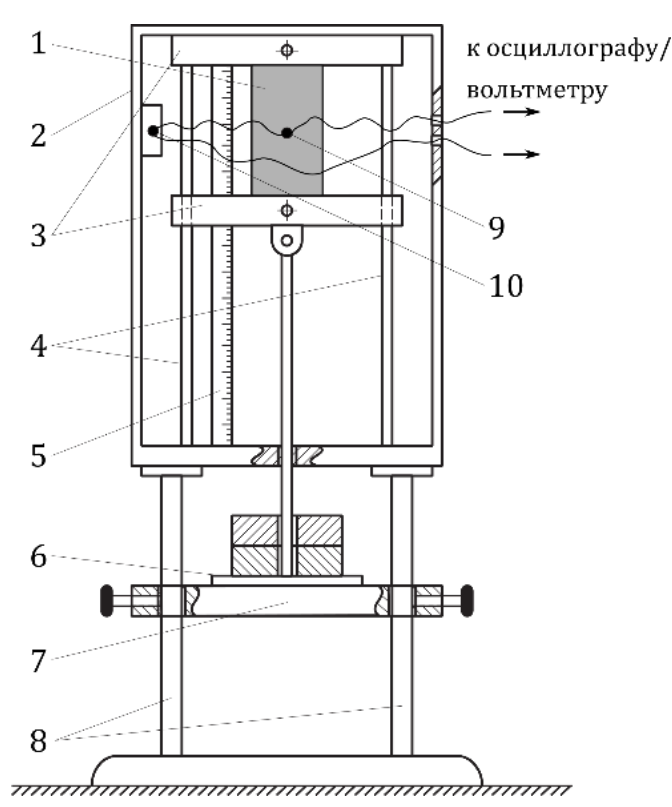
\includegraphics[width=0.5\textwidth]{Установка}
\end{center}
\caption{Схема экспериментальной установки} \label{установка}
\end{figure}
Измерять изменение температуры при адиабатическом растяжении можно двумя способами: быстро растянуть резину и измерить скачок (возможно возникновение необратимых эффектов) и медленно растягивать резину и экстраполировать резину к начальному моменту (возникает ошибка неизвестная ошибка экстраполяции).
\begin{figure}[h!]
\begin{center}
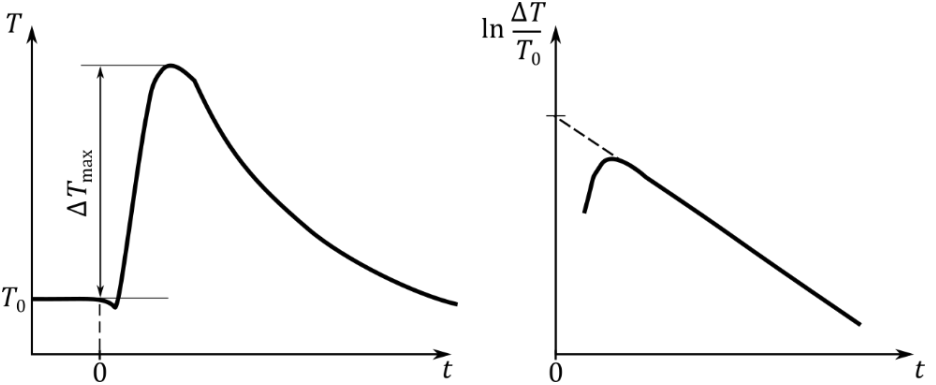
\includegraphics[width=0.5\textwidth]{Измерение}
\end{center}
\caption{Измерение термического эффекта от растяжения по зависимости от времени} \label{измерение}
\end{figure}
\newpage
\section{Измерения и обработка данных}
Начальные размеры образца представлены в таблице \ref{база}.
\begin{table}[h!]
\caption{Начальные параметры установки} \label{база}
\begin{tabular}{|l|l|l|l|}
\hline
$l_0$, см      & $d_0$, мм      & $h_0$, мм       & $\rho$, г/$см^3$ \\ \hline
$10.7 \pm 0.1$ & $12.0 \pm 0.5$ & $1.80 \pm 0.05$ & 1.2              \\ \hline
\end{tabular}
\end{table}
\subsection*{Растяжение резины от нагрузки}
Результаты измерений растяжения при разных нагрузках представлены в таблице \ref{f(l)_tab} и на графике \ref{f(l)_pic}.

\begin{table}[h!]
\caption{Растяжение резины при разных подвешенных грузах } \label{f(l)_tab}
\begin{tabular}{|l|l|l|l|l|l|l|l|l|}
\hline
$m_{грузов}$, г      & 176.7 & 354.8 & 529.6 & 707.7  & 872.7 & 1078.3 & 228.9 & 407 \\ \hline
$\Delta l$, мм & 6     & 13    & 26    & 38     & 58    & 82     & 8     & 18  \\ \hline \hline
$m_{грузов}$, г       & 581.8 & 759.9 & 924.9 & 1130.5 & 529.6 & 706.3  & 884.4 &     \\ \hline
$\Delta l$, мм  & 31    & 48    & 66    & 87     & 27    & 44     & 62    &     \\ \hline
\end{tabular}
\end{table}

\begin{figure}[h!]
\begin{center}
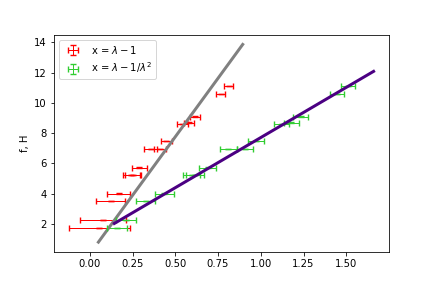
\includegraphics[width=\textwidth]{f(l)}
\end{center}
\caption{Зависимость силы от растяжения в двух моделях: закон Гука и модель идельной полимерной сетки} \label{f(l)_pic}
\end{figure}
Из графиков и начальных значений установки можно найти значение модуля Юнга резины:
\begin{table}[h!]
\caption{Значение модуля Юнга}
\label{юнг}
\begin{tabular}{|l|l|l|}
\hline
                  & Идеальная полимерная сетка & Закон Гука \\ \hline
E, МПа            & 0.92                       & 0.72       \\ \hline
$\sigma_E$, МПа   & 0.02                       & 0.11       \\ \hline
$\varepsilon$, \% & 2                          & 15         \\ \hline
\end{tabular}
\end{table}


Исходя из значений погрещности модуля Юнга (табл. \ref{юнг}) для закона Гука и из вида графика заметно, что резина плохо подчиняется закону Гука. При этом модель идеальной полимерной сетки достаточно точна.

Для теоретической модели растяжения резины:
\begin{equation}
f(T, \lambda) = s_0E\cdot \frac{1}{3}(\lambda-\frac{1}{\lambda^2}
\end{equation}
Можно вычислить работу от растяжения:
\begin{equation}
\label{A}
A(\lambda) = \frac{1}{3}s_0E(\frac{\lambda^2}{2}+\frac{1}{\lambda}-\frac{3}{2})
\end{equation}



\subsection*{Измерения при быстром растяжении резины}
Данные в таблице \ref{fast_tab}. 
\begin{table}[h!]
\caption{Зависимость изменения напряжения от растяжения}
\label{fast_tab}
\begin{tabular}{|l|l|l|l|l|l|l|l|l|l|l|l|l|l|l|l|}
\hline
$\Delta l$, мм & 93  & 103 & 103 & 74  & 74  & 61 & 57 & 47 & 47 & 40 & 40 & 36 & 36 & 26 & 26 \\ \hline
$\Delta V$, мВ & 168 & 206 & 206 & 126 & 129 & 90 & 86 & 60 & 62 & 48 & 48 & 40 & 40 & 22 & 24 \\ \hline
\end{tabular}
\end{table}


\subsection*{Зависимость температуры от времени при абиабатическом растяжении}
Зависимость напряжения от времени представлена в таблице \ref{slow_tab}. Данные собирались с графиков от осциллографа, например, \ref{осциллограф}. По полученным данным построим график логарифма приращения температуры от времени \ref{T(t)}.



\begin{table}[h!]
\caption{Зависимость температуры от времени}
\label{slow_tab}
\begin{tabular}{|ll||ll||ll|}
\hline
\multicolumn{2}{|l|}{$\lambda = 1.87$} & \multicolumn{2}{l|}{$\lambda = 1.96$} & \multicolumn{2}{l|}{$\lambda = 1.69$} \\ \hline
\multicolumn{1}{|l|}{V, мВ}   & t, с   & \multicolumn{1}{l|}{V, мВ}   & t, с   & \multicolumn{1}{l|}{V, мВ}   & t, с   \\ \hline
\multicolumn{1}{|l|}{-70}     & -39    & \multicolumn{1}{l|}{-48}     & -39    & \multicolumn{1}{l|}{-55}     & -39    \\ \hline
\multicolumn{1}{|l|}{108}     & -34    & \multicolumn{1}{l|}{158}     & -35    & \multicolumn{1}{l|}{71}      & -35    \\ \hline
\multicolumn{1}{|l|}{97}      & -30    & \multicolumn{1}{l|}{146}     & -30    & \multicolumn{1}{l|}{67}      & -30    \\ \hline
\multicolumn{1}{|l|}{75}      & -20    & \multicolumn{1}{l|}{111}     & -20    & \multicolumn{1}{l|}{44}      & -20    \\ \hline
\multicolumn{1}{|l|}{53}      & -10    & \multicolumn{1}{l|}{89}      & -10    & \multicolumn{1}{l|}{32}      & -10    \\ \hline
\multicolumn{1}{|l|}{42}      & 0      & \multicolumn{1}{l|}{72}      & 0      & \multicolumn{1}{l|}{24}      & 0      \\ \hline
\multicolumn{1}{|l|}{33}      & 10     & \multicolumn{1}{l|}{54}      & 10     & \multicolumn{1}{l|}{14}      & 10     \\ \hline
\multicolumn{1}{|l|}{24}      & 20     & \multicolumn{1}{l|}{47}      & 20     & \multicolumn{1}{l|}{8}       & 20     \\ \hline
\multicolumn{1}{|l|}{19}      & 30     & \multicolumn{1}{l|}{33}      & 30     & \multicolumn{1}{l|}{4}       & 30     \\ \hline
\multicolumn{1}{|l|}{10}      & 40     & \multicolumn{1}{l|}{26}      & 40     & \multicolumn{1}{l|}{}        &        \\ \hline
\end{tabular}
\end{table}

\begin{figure}[h!]
\begin{center}
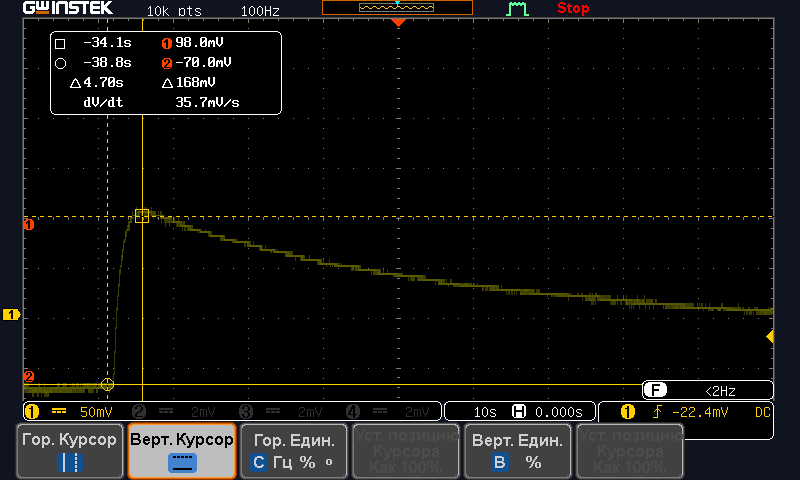
\includegraphics[width=\textwidth]{DS0002}
\end{center}
\caption{Пример графика от осциллографа для $\lambda = 1.87$} \label{осциллограф}
\end{figure}

\begin{figure}[h!]
\begin{center}
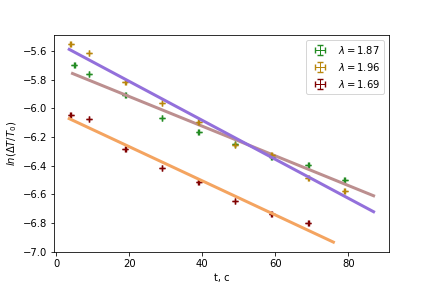
\includegraphics[width=\textwidth]{T(t)}
\end{center}
\caption{зависимостей логарифма приращения температуры $ln \frac{\Delta T}{T_0}$
от времени t} \label{T(t)}
\end{figure}

Экстраполируем зависимость на начальный момент времени, данные в таблице \ref{экстраполяция}.

\begin{table}[h!]
\caption{Экстраполяция зависимости температуры от времни на начальные значения}
\label{экстраполяция}
\begin{tabular}{|l|l|l|l|}
\hline
$\lambda$              & 1.87 & 1.96 & 1.69 \\ \hline
$\Delta T$, K          & 0.90 & 1.07 & 0.66 \\ \hline
$\sigma_{\Delta T}$, K & 0.03 & 0.03 & 0.03 \\ \hline
$\varepsilon$, \%      & 3.3  & 2.8  & 4.5  \\ \hline
\end{tabular}
\end{table}

\subsection*{Вычисление параметров резины}
Из таблицы \ref{экстраполяция} и \ref{fast_tab} построим график зависимости $\Delta T$ от А, используя формулу \ref{A}. (рис. \ref{T(A)_pic})

\begin{figure}[h!]
\begin{center}
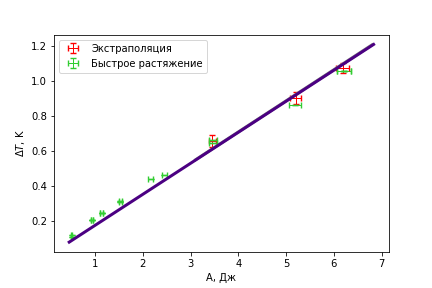
\includegraphics[width=\textwidth]{T(A)}
\end{center}
\caption{Зависимость $\Delta T$ от A в двух моделях: закон Гука и модель идельной полимерной сетки} \label{T(A)_pic}
\end{figure}

Из графика найдем теплоемкость и удельную теплоемкость резины \ref{теплоемкость}
\begin{table}[h!]
\caption{Теплоемкость резины}
\label{Теплоемкость}
\begin{tabular}{|l|l|l|}
\hline
                  & Быстрое растяжение & Экстраполяция   \\ \hline
$С_l$, Дж/К       & $5.66 \pm 0.18$    & $5.64 \pm 0.29$ \\ \hline
$\varepsilon$, \% & 3.1                & 5.1             \\ \hline
$c_l$, Дж/К/кг    & $2040 \pm 66$    & $2034 \pm 105$ \\ \hline
$\varepsilon$, \% & 3.2                & 5.2             \\ \hline
\end{tabular}
\end{table} 

В обоих методах вышли похожие значения, табличное для удельной теплоемкости: $c_l = 1886 Дж/К/кг$.


\section{Выводы}

1. Проверили разные модели описания растяжения резины, для модели идеальной полимерной решетки получили значение модуля Юнга: $E = 0.92 \pm 0.02 МПа$, табличное значение $\sim 1 МПа$, что согласуется с полученным результатом.

2. Разными методами: экстраполяцией медленного процесса и измерением при быстром растяжении получено значение удельной теплоемкости резины $c_l = 2040 \pm 66 Дж/К/кг$, что близко к табличному значению $c_l = 1886 Дж/К/кг$.
\end{document}